\documentclass[review,twocolumn,5p]{elsarticle}

% Packages Import
%\usepackage[utf8]{inputenc}
%\usepackage{mathptmx}
%\usepackage{algpseudocode}
%\usepackage{algorithm}
\usepackage{mathtools}
\usepackage{url}
\usepackage{enumerate}
%\usepackage{verbatim}
%\usepackage{diagbox}
%\usepackage{eucal}
%\usepackage{lipsum}
%\usepackage{titlesec}
%\usepackage{amsfonts}
%\usepackage{amsthm}
\usepackage{multirow}
\usepackage{sidecap}

\biboptions{longnamesfirst,semicolon}

\begin{document}


\begin{frontmatter}

% Title
\title{Stock index prediction model using financial news documents in a dynamic feature space}
\author[rvt]{Saurav Das\corref{cor1}}
\ead{saurav.das37@gmail.com}
\author[rvt]{S.G.Sanjeevi\corref{cor2}}
\ead{sgs@nitw.ac.in}
\address[rvt]{National Institute of Technology, Warangal - 506004, India}
\date{}

\begin{abstract}
Stock market prediction based on financial news has been studied previously by various researchers using varied methodology. In our study, we noted that the changing news and concept-drift in the market can affect the static feature space prediction methods used in other models. Hence, we explore a dynamic feature space to correctly represent the changing concepts and their effects in the market. We design a prediction model that uses the changing feature space, classifies the new news articles and then uses an Artificial Neural Network to predict the BSE S\&P 500 Sensex index. A profitable intra-day trading system has also been developed to get us better returns for trader investment. 
\end{abstract}
\begin{keyword}
Text Mining \sep Financial prediction \sep News classification
\end{keyword}
\cortext[cor1]{Corresponding Author}
\cortext[cor2]{Research Supervisor}
\end{frontmatter}
\section{Introduction}
\label{sec:introduction}

Stock market has been a field of interest for businessmen, common people and researchers as well for many years. Several methods has been adopted and designed for predicting the stock market values. These predictions help trader make better decisions regarding the trading of stocks. News coverage by the media carries much information regarding the current trends of a market. For each development the on-line news stream provides live coverage. These news motivates or gets people away from stocks of particular kind. Thus news articles have a wide potential in changing the market. So it can be used to determine the trend in the market. This has been the basic theory by several researchers who have predicted trends in the market according to the recent news developments.

Since the advent of Internet and strong networking, there is a large content of data in the form of news available. Stock traders use these sources to make trading decisions and this affect the market. So, an automated system which can predict the change in market due to some news would give us the same effect as an experienced stock trader.

Text mining methods is used to classify news and predict news sentiments. However popular methods have already found out that the sentiment of an article is not of main relevance here. In a particular context some article which may contain negative words may also have reason to cause stock market to rise. So normal classification techniques can't be used, and modified techniques should be used to evaluate the news articles.

Existing research regarding this field has developed ways to mine the content in the news articles and formulate effective methods of trading according to the news. Hagneau et al. in \cite{Hagenau:2013} has formulated good feature extraction techniques which give much more representative features to represent documents. The AZFinText model developed by Schumaker et al. in \cite{Schumaker:2009} is also an important model used for predictions.

Our motivation for the research was based on capturing the change in the underlying concept, and how news features keep changing with time and in case of financial market the most recent news may contain some trend capturing context which was preciously not there during the training phase of the models. So a dynamic training with feature set up-gradation is necessary for the effective understanding of the underlying semantics of news articles. We design a prediction model that uses the changing feature space, classifies the new news articles and then uses an Artificial Neural Network to predict the BSE S\&P 500 Sensex index. A profitable intra-day trading system is developed to get us better returns for trader investment. 

The rest of the paper has been organized in several sections. Section 2 discusses some of the theories regarding stock market predictions and the different existing researches in this field. In section 3, we talk about the questions which drive this research and the approaches used by the model designed by us. Section 4 we discuss the experiments set-up to verify the working of our prediction model on real data set. In Section 5, we summarize our approach and future ways to develop the model has been talked about. 


\section{Related Works}
\label{sec:related-works}

There has been a lot of work in the field of stock market prediction. The two prevalent theories are The Efficient Market Hypothesis (EMH) and the Random Walk Theory (RWT). In finance, the Efficient Market Hypothesis (EMH), or the Joint Hypothesis problem, asserts that financial markets are "informationally efficient". The random walk hypothesis is a financial theory stating that stock market prices evolve according to a random walk and thus cannot be predicted.

Though the Efficient Market Hypothesis and Random Walk Theory say that stock values cannot be predicted, researchers do not agree to this theory. Several counter theories and models have been designed which has been seen to provide considerable amount of gain in the market. The semi-strong-form efficiency of the market is used along with the rapid analysis of information to give hint as to which direction the market is going. Machine learning techniques help in this process. 

Our project is mainly concerned about the change in the stock market index. The prediction of stock market index with financial news as aid, which gives us hints about which way the stock market is being driven to. 

The basic strategy of news based trading is to buy or sell stocks according to the market news. But this is not applicable always, because sometimes the news in the market is already anticipated so even a good news does not have that much difference in the stock market prices as the effect is slowly dissolved in the market and the market has adjusted itself in anticipation. Best changes are found out due to the breaking news which cause the drop or rise in market values. 

Stock trading has been affected due to economic news publications \cite{RePEc:eee:pacfin:v:9:y:2001:i:3:p:195-217}. However not always can the financial news correctly predict the market changes, because other factors are still relevant in the market. There are also sudden unforeseen rise and fall of prices in the market because of large amount of trades \cite{camerer1991information}. 

Many researchers have worked on this concept and many different models have been designed which deal with time series stock market prediction. The data set which has been used in prediction comprises of the financial message base and the stock market change after this news item is released. The financial message base may contain financial news articles as used in \cite{Schumaker:2009}\cite{JOFI:JOFI1362}\cite{1265201}, ad-hoc corporate announcements as used in \cite{conf/wirtschaftsinformatik/GrothM09}\cite{groth2011intraday}, worldwide general news as used in \cite{725072}, corporate filings as used in \cite{JOAR:JOAR382}, message postings as used in \cite{doi:10.1287/mnsc.1070.0704} or annual reports as in \cite{butler:2009}.

The financial news obtained have to be correctly processed and represented in a format which can help machine learning algorithms properly analyze the data and train accordingly. Text mining on the news body is done for feature processing. Feature processing comprises of 3 steps -

\begin{enumerate}
\item Feature Extraction

In this step the type of features which are used to represent the documents are defined. Features are extracted accordingly which best reflect the content of the documents. Many different approaches of feature extraction has been used by different researchers such as bag-of-words \cite{conf/wirtschaftsinformatik/GrothM09}\cite{1265201}\cite{725072}\cite{JOAR:JOAR382}\cite{antweiler2004all}, noun phrases \cite{Schumaker:2009}, n-grams \cite{butler:2009}, 2-word combinations \cite{Hagenau:2013}. 

\item Feature Selection

In the feature extraction step many features are generated which are not all important and maximum of them comprise of redundant features. We need to take a subset of the features extracted which will give us the best features to represent the documents. Different feature selection methods used are - Dictionary based \cite{JOFI:JOFI1362} and Exogenous market feedback \cite{groth2011intraday}\cite{Hagenau:2013}. Chi-Square and Bi-Normal Separation are statistical methods which are used for the selection process.

\item Feature Representation

Documents need to be represented in machine readable format so that machine learning algorithms can be applied on them. Feature representation is the step of converting the documents to machine readable format so that learning algorithms can train themselves on these document vectors and make future predictions. 
\end{enumerate}
After the feature processing is completed and the documents of the data set are converted in machine readable format machine learning algorithms are applied on them. The stock market prediction is the correct prediction of the trend of the market. This is achieved by training the machine using various algorithms. Many different algorithms have been used by the researchers. Support Vector Machine (SVM) is a very popular method in \cite{Schumaker:2009}\cite{conf/wirtschaftsinformatik/GrothM09}\cite{1265201}. Na\"{i}ve Bayes has been used in \cite{725072}. A combination of Bayes and SVM has been used in \cite{antweiler2004all}, Ratio of negative words has been used in \cite{JOFI:JOFI1362}. Propriety distance measures has been used in \cite{butler:2009}. The classification accuracy is the main metric which is examined to determine how well the news is being classified. 

Some of the popular stock prediction architectures already present, which have good returns are the NewsCATS method which was designed by Mittermayer \cite{1265201}. Uses bag-of-words feature and SVM for the classification of the news documents. Another very famous architecture is the AZFinText which was designed by Schumaker \& Chen \cite{Schumaker:2009}. This uses proper nouns as features and SVR for the stock price prediction. A new method has been designed by Hagneau et al. \cite{Hagenau:2013}. This uses a new kind of feature called 2-word combination. The method by Hagneau et al. has shown better classification accuracy than other methods.

\section{Research Design}
\label{sec:research-design}

From the related work we get a brief view of the methodologies used by previous researchers to design a profitable trading system. Our research goals and objectives lies in finding scope for improvement in the related work. 

\subsection{Research Questions}
There are 3 major questions which are the base of our further research - 
\begin{enumerate}
\item \textbf{Question} : Does a fixed feature space capture all trends of the stock market?

\textbf{Answer} : The classification or regression models used by the researchers previously all have a static feature space and when some new item comes those specific features are searched and the new item is classified accordingly. The concept drift in the data is not considered in these methods.

The determining factors of financial news is ever changing. There are always new buzzwords in the market which are determinants of the stock market. For a financial market, a company when is on loss can fall under negative determinant while if the same company sees boost in market, perhaps due to some acquisition then the company name can be considered as a positive determinant. 

A fixed feature space won't be able to capture these recent trends in the stock market, because it's features will always be limited to the trends predominant in the time the model was trained. And if the model is trained according to news data which are widely spanned, then they will capture the most generalized trends of the market. Since we are concerned about intra-day predictions, thus features conveying short changes in market would be more helpful. 

\item \textbf{Question} : How little can training phase be for the prediction of stock data?

\textbf{Answer} : Generally extensive training of prediction models are done before the model is actually used. But is extensive training always effective and necessary? Extensive training may lead to over-fitting of training data. Also, training according to some very old data will only give us old trend features. In the stock market there's always new trends and new features to determine them.

\item \textbf{Question} : Can a trading strategy be defined by using the Index values?

\textbf{Answer} : The previous researches have all developed a trading strategy based on the prediction of the stock price of a specific stock. However in our research we strategize to trade according to the S\&P BSE Sensex Index. The BSE index correctly reflects the current market conditions. The index is calculated based on a free float capitalization method, a variation of the market capitalization method. In short term intra-day trading thus the market index can help us understand the total market situation better. In stock markets, chaining effects does take place which means that the effect in one stock can cause simultaneous effect in other stocks of related field. So, an overall effect analysis may possibly cause better trading and increased returns. 
\end{enumerate}

\subsection{Solutions proposed}
\begin{enumerate}
\item \textbf{Problem} : Fixed feature space doesn't capture recent trends

\textbf{Solution} : A dynamic feature space would be much better for capturing recent trends. The conversion of a static feature space to a dynamic feature space is done according to the lossless homogeneous feature space conversion. We will discuss about the lossless homogeneous feature space conversion later. The new documents are classified by clustering of the points. However, the dynamic feature space conversion increases the feature space size considerably and thus dimensionality of the document vectors also increases. This causes a problem as it is difficult to classify high dimensional data points because they tend to become equidistant from each. The distance to the nearest data point is similar to the distance to the furthest point \cite{Beyer:1999} and this can be attributed to the 'curse of dimensionality'. 

\item \textbf{Problem} : For high dimensional data due to sparsity of data points, all points tend to become equidistant from each other.

\textbf{Solution} : The problem faced by the feature space conversion is that it causes the points in the feature space to become equidistant from each other. The high dimensional feature space prevents proper clustering of data points due to the sparsity of data points. This can be solved by using methods like - subspace clustering or projected clustering. We use projected clustering because of it's quick computation and less management of different subspaces.
\end{enumerate}

\subsection{Approach Overview}
The approach used in our work is briefly defined here. The main training base for our project are the financial news articles. News articles are classified into 3 classes - 'positive', 'negative' and 'neutral'. The 'positive' class defines those articles that will boost the stock market, the 'negative' class contains articles which will cause a degradation of stock prices and the 'neutral' class has minimal effect on the stock market.

The 2 main phases of our findings are - 

\begin{enumerate}
\item \textbf{ANN training phase}

In this phase data is collected for training of the Artificial Neural Network (ANN) model which is used later for the prediction of the stock price. The ANN model takes in the change in the stock market index in the previous 15 minute time frame along with other financial parameters and news sentiments and then predicts the change in the next 15 minutes.

\item \textbf{Market Prediction phase}

For our model the only pre-training is done on the previous data. The features which would form the feature space for classification are chosen dynamically. Initially a feature space is defined using the news items from the previous day. The news items from the previous trading day form the initial clusters. Any new news which comes is classified using projected clustering. After the news at a particular time is classified into a particular sentiment class it is fed into the ANN along with other factors as a parameter to determine the movement of the stock index.
\end{enumerate}

\subsection{Data Acquisition}
\label{sec:ann_parameters}
For our prediction purpose we need financial news and stock market data. The financial news articles are collected from various popular news sites and labelled according to the exogenous market feedback as done in \cite{Hagenau:2013}. This method has been proved to be better because it gives us the most relevant features differentiating between the different classes of news. The different classes taken are - positive, negative and neutral. 

Our approach of labelling is as follows - as the news articles are released the stock price change is noted every 5 minutes. A total of 15 minutes time window is kept for the news affecting the stock market. The 15 minute window is divided into 5 minute intervals. 50\% importance is given to the change in the first 5 minutes. 30\% importance to the second 5 minutes and 20\% importance is given to the last 5 minutes.
 
\begin{equation}
\begin{array}{ll}
change_{total} = & ( bsechange_{1} ) \times 0.5 + ( bsechange_{2} ) \times 0.3 \\
    & + ( bsechange_{3} ) \times 0.2 \\
\end{array}
\end{equation}
$change_{total}$ : Total change in the 15 minute window \\*
$bsechange_{1}$ : The change in the first 5 minutes \\*
$bsechange_{2}$ : The change in the second 5 minutes \\*
$bsechange_{3}$ : The change in the last 5 minutes \\*

This gives maximum importance to the change in the first 5 minutes and gradual decrease in the change importance. The labelling of the documents is done as follows - 

\begin{equation}
sentiment=
	\begin{cases}
		positive, & \text{if}\ change_{total} \geq change_{threshold} \\
		negative, & \text{if}\ change_{total} < 0.0 \\
     	neutral, & \text{otherwise}
	\end{cases}
\end{equation}

The $change_{threshold}$ is taken as 5.0. News articles which cause more than 50\% increase or decrease in the values of stock are considered as positive or negative news respectively. The other news items are however considered as neutral, making minimum changes which is inherent in stock markets and can't be really attributed to some change caused due to news. 

There are other parameters which are considered when predicting the stock price movements. The following factors are primarily considered as parameters affecting the Indian market according to \cite{ghosh:2010}. Crude Oil price, Gold price, Cash Reserve Ratio, Food price inflation, Call money rate, Dollar price, FDI, Foreign Portfolio Investment and Foreign Exchange Reserve (Forex). Since we are predicting the intra-day stock price changes we consider those components whose values change intra-day. The Cash Reserve Ratio, Food price inflation, Call money rate, FDI, Foreign Portfolio Investment and Foreign Exchange Reserve (Forex) are economic determinants but they change quarterly or monthly. So, they are not considered. Only Crude Oil price, Gold price, Dollar Exchange rate changes are considered in our model. 


\subsection{Preparation of News articles}
After the news articles have been gathered by our collector and before the news article is used for classification prediction or classifier training the news article needs to be pre-processed properly and made ready for the machine learning algorithm to be applied on it. 

The various steps required for the preparation of the news articles are - 
\begin{enumerate}
\item  \textbf{Document Pre-processing} : Removal of punctuation marks, numbers, stop-words and symbols. Tokenizing of the text. Stemming of the words using the Porter Stemmer algorithm \cite{porter1980algorithm}. 

\item \textbf{Feature Extraction} :  We extract 2-word combination feature as defined by \cite{Hagenau:2013} for our work.

\item \textbf{Feature Selection} :  The explanatory power of the features are determined by the statistical method of Bi-Normal-Separation (BNS). The BNS selection method determines the prevalence of a feature in a specific class rather than in the rest classes. The BNS formula we use is defined as - 
\begin{equation}
\label{eq:bns}
BNS_{i} = max \left\{ F^{-1} \left(\frac{O_{i,x}}{|x|}\right) - \sum_{y \in \{S - x\}} F^{-1} \left(\frac{O_{i,y}}{|y|}\right)  \middle| x \in S \right\}
\end{equation}
where, $S = \{ positive, negative, neutral \}$ are the different sentiment classes. $F^{-1}$ is the standard normal distribution's inverse normal cumulative probability function or z-score. $O_{i,x}$ denotes the observed frequency of the number of instances of the occurrence of feature $i$ in the class x documents. The value of $F^{-1}(0)$ is substituted by 0.0005 \cite{Forman:2003}.

\item \textbf{Document Representation} : After the feature selection is done we get a feature space. This feature space is used to create the document vectors as in Vector Space Model. A particular document $D_{j}$ is represented as - 
\begin{equation}
d_{j} = ( w_{1,j} , w_{2,j} , ... , w_{n,j} )
\end{equation}
where, $w_{i,j}$ is the weight of feature $i$ in document $j$. $n$ is the total number of features present in the feature space. 

The features which are not present in the document are given zero weight-age. The weight metric selected for our study is TF-IDF measure.
\end{enumerate}



\subsection{Lossless Homogeneous Feature Space Conversion}
\label{sec:lhfs}

Every time we come across a new news document we collect new features from the document. In our work a dynamical feature space is being considered to deal with the problem of capturing the recent stock market buzzwords. Lossless Homogeneous feature space conversion has been used to change the feature space in \cite{Masud:2010}. Each time we select 40 new features to add to the existing feature space. We use a modified version of the feature space conversion technique to suit our needs better. 

The steps for the feature space conversion are as follows - 
\begin{enumerate}
\item A block of the most recent news articles are kept containing the last 10 news articles released before the release of the present news article. From this block of news articles we extract and select the best 1000 features according to the 2-word combinations and BNS techniques respectively.

\item From the new news documents we extract all the 2-word combinations as features.

\item The features set we got from the new news articles and the feature set selected from the most recent news articles intersect to form a set of features. 60\% of the extended feature set are added from this intersection set. 

\item The features in the new articles which are completely new, not present previously in any news articles form a new set of features. These features are ranked according to the frequency of their occurrence in the news articles. The most frequent features make up the rest 40\% of the extended feature set. 
\end{enumerate}

\subsection{Fading Cluster}
\label{sec:fading}
The news data stream which we have consists of multiple data points in a time. The Fading Clusters concept for handling data points in a data stream has been introduced in \cite{Aggarwal:2005} to provide more importance to the most recent data points. Each data point has a weight assigned to it according to the fading function $f(t)$ whose value lies between (0,1). The fading function is a monotonically decreasing exponential function which decays uniformly with time $t$. The fading function $f(t)$ is defined as- 
\begin{equation}
f(t) = 2^{-\lambda \cdot t}
\end{equation}
where, $\lambda$ is the decay-rate and is defined as the inverse of the half-life of the data stream and t is the time at which the data point came to the data stream. Thus, $\lambda = 1/t_{0}$, $t_{0}$ being the half-life time for data points.


For projected clustering of the data points, with each of the fading cluster assigned a d-dimensional bit-vector $B(C)$. This bit-vector tells which dimensions are relevant for the cluster. Each entry of the bit-vector corresponds of 0 or 1. 0 representing the dimension is not relevant for the cluster and 1 otherwise. 

\subsection{Projected Clustering}
\label{sec:proj_clustering}
The algorithm for Projected Clustering on data streams has been designed in the HPStream algorithm by Charu et al. \cite{Aggarwal:2005} and is used by us to classify the incoming news.

Let us consider that we have a Fading Cluster Structure (FCS) which is denoted as $FCS = \{ FC^x(C_1, t), ... , FC^x(C_n, t)\}$. The Dimensionality Vector Set $B(S)$ containing information about the relevant dimensions for a cluster is denoted as - $B(S) = \{ B(C_1), ... , B(C_n)\}$. Now at current time $t$ a new data point $X$ arrives. We need to put this new data point in the proper cluster. 

Initially a full-dimensional clustering using k-means is performed. The data points are assigned to the newly formed clusters according to the distance of the data points from the cluster centres considering only the relevant dimensions. After putting the data points into new clusters, again the relevant dimensions of the clusters according to the data points are evaluated. This process continues until the clusters set converges. 

The steps which are done to classify the news are - 
\begin{enumerate}
\item \textbf{Conversion of feature space}

Lossless Homogeneous Feature Space conversion is done as specified in section~\ref{sec:lhfs}. It gives us the new feature space. As soon as the feature space changes the new features have to be added to all the clusters present in the Fading Cluster Structure. They are marked irrelevant for the existing clusters as they are the new features and wouldn't affect the old values which were not dependent on these new features. 

\item \textbf{Compute new dimensions for each cluster}

For each of the cluster we need to find the most relevant dimensions after the addition of the new news item $X$. This is done because the relevant dimensions of a cluster tell us which of the dimensions bind the cluster together most and not allow it to spread over a large area carrying outliers. 

The new data point $X$ is added to all the existing clusters. This is done specially because in the worst case some clusters may contain only one point and for these clusters it is difficult to find the spread along each dimension. The dimensions which are selected are such that new point $X$ fits when added to the cluster.

The spread radius $r_j^i$ is calculated for all the $d$ dimensions of each fading cluster according to the equation given in \cite{Aggarwal:2005}.

If the average number of relevant dimensions per cluster is $l$, then the minimum $|FCS| \times l$ dimensions are selected from among the $|FCS|*d$ according to the least spread radius. 

Once the selected dimensions are chosen the bits chosen corresponding to the relevant dimensions are stored in the vector $B(S)$.

\item \textbf{Projected Distance of new point from clusters}

The Manhattan Segmental Distance is used as the measure for distance. For each of the clusters in the faded cluster structure, we find the distance between the respective cluster center and the new data point along the relevant dimensions. The relevant dimensions are found according to the vectors in $B(S)$. The cluster which has minimum Manhattan Segmental distance from the cluster center to the new point is chosen as the cluster where the new data point should be put into. 

\item \textbf{Determine limiting radius of chosen cluster}

The Limiting Radius is considered as the natural boundary of the cluster. If the point lies within this radius then it is put into the cluster else the point forms a new cluster. 

The radius $r_j, \forall j \in D$ is calculated according to the equation \ref{eq:spread_radius}. The relevant radius $R$ of the cluster $C_i$ is given as -
\begin{equation}
R_i = \sqrt{ \frac{\sum_{j \in B(C)} r_j^2}{d'} }
\end{equation}
where, d' is the number of bits having value 1 in $B(C_i)$.

This value is scaled by a boundary factor $\tau$ to determine final value of limiting radius. 

\begin{equation}
R = R \times \tau
\end{equation}

\item \textbf{Add new data point to cluster}

The new data point is added to the new cluster and the cluster information is updated. Every time before the addition of a new data point, the exponential decay of the elements weight takes place. This is done by using the temporal multiplicity property of the Fading Clusters. The last time a cluster is updated is stored for each cluster. Let, $t$ be the current time and $t_{up}$ be the last time the cluster was updated. Then a factor of $e^{- \lambda \cdot (t-t_{up})}$ is multiplied with each of the statistics stored for the fading cluster. 

After the weight decay is done, according to the additive property of the fading clusters the weight values are added to the cluster statistics. The second order and first order temporal weights are calculated. The cluster center is recalculated, and the last time the cluster was updated is set as time now, i.e. $t_{up} = t$.

\item \textbf{Cleanup of unused clusters}

The fading projected clusters which have no relevant dimensions assigned to them are removed from the fading cluster structure. These clusters don't provide relevant information anymore according to the current time. 

If the number of clusters present at a particular time increases than a maximum number of clusters then the cluster which has been updated least recently is removed from the cluster set. 
\end{enumerate}

\subsection{Classification of data points}

A majority voting scheme is carried out to classify the new data point into a specific cluster. We keep the spread radius less to make the clusters for each class small. This helps in stopping misclassification of data.

\subsection{ANN model}
\label{sec:ann}
The ANN model we use in our project has been used in \cite{kohara:1997}. This ANN model uses the event knowledge and other parameters to calculate the effect on the stock prices. However Kohara et al. uses \textit{Prior Knowledge} to predict the \textit{event knowledge} for the current news. Our approach differs in the way that we predict the news sentiment of the news article using our classification method and use it as \textit{event knowledge}. 

\subsubsection{Inputs to ANN}

The different parameters we use for our prediction has already been discussed in section \ref{sec:ann_parameters}. The output for the neural network is the change in the stock index for the next window of 15 minutes. 

The inputs to the neural network are - 
\begin{enumerate}
\item Change in BSE index value for the previous time interval
\item Change in the dollar-to-rupee exchange rate for the previous time interval
\item Change in the crude oil price per barrel rate for the previous time interval
\item Change in the gold rate for the previous time interval
\item Sentiment of the news articles released in the time interval
\end{enumerate}

\subsubsection{Pre-processing of data}
Before the training phase of the network, the input parameters are normalized using z-score normalization method. The targets outputs are normalized during training, by the \textit{min-max normalization}. 

\subsubsection{Training and convergence}
\label{subsec:training}

We use backpropagation to train our neural network. The convergence of the weights is determined by taking the error on the 5 cross validation set. 

\begin{table*}[!t]
\centering
\caption{ANN normalized error}
\label{tab:error}

\vspace{15pt}
\begin{tabular}{|l|l|l|l|l|l|l|}
\hline
\multirow{2}{*}{Activation Function} & \multicolumn{3}{c|}{$\lambda$ = 0.5}                                                      & \multicolumn{3}{c|}{$\lambda$ = 0.05}                                                  \\ \cline{2-7} 
                  & \multicolumn{1}{c|}{$h$ = 3} & \multicolumn{1}{c|}{$h$ =2} & \multicolumn{1}{c|}{$h$=1} & \multicolumn{1}{c|}{$h$=3} & \multicolumn{1}{c|}{$h$=2} & \multicolumn{1}{c|}{$h$=1} \\ \hline
Log Sigmoid       & 0.30865                    & 0.30154                   & 0.28158                  & 0.28199                  & 0.2815                   & 0.28136                  \\ \hline
Bipolar Sigmoid   & 18.428                     & 18.42799                  & 18.42799                 & 18.42802                 & 18.42799                 & 18.42799                 \\ \hline
Tan Hyperbolic    & 18.42128                   & 18.42799                  & 18.42712                 & 18.42794                 & 18.42783                 & 18.42807                 \\ \hline
\end{tabular}
\end{table*}


\subsubsection{Activation Function}
\label{subsec:activation}
The different kinds of activation functions that we use for our study are - 
\begin{enumerate}
\item Continuous Log-Sigmoid Function
\item Continuous Bipolar Log-Sigmoid Function
\item Continuous Tan-Sigmoid Function
\end{enumerate}

\section{Experimental Results}
\label{sec:expt-results}

\subsection{ANN model}

The different parameters which we change in the ANN are - number of hidden units used, the learning rate and according to the different activation functions as mentioned in \ref{subsec:activation}. The normalized errors generated are presented in table-\ref{tab:error}. In the table $\lambda$ is the learning rate and $h$ denotes the number of hidden used in the ANN network. 


From the table-\ref{tab:error} we can see that the sigmoid activation function is the best for our data since it gives the least error. The number of hidden units taken is 1. 

The change in error with the training iterations for the least error configuration as found out is given in figure-\ref{fig:error_plot}.

\begin{figure}[h]
\centering
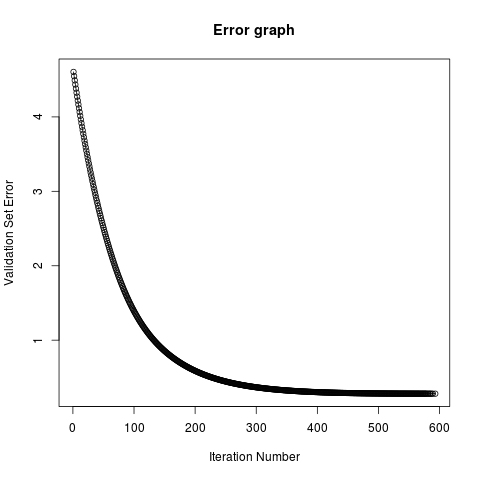
\includegraphics[scale = 0.5]{pictures/errorPlot.png}
\caption{Change in Error over iteration}
\label{fig:error_plot}
\end{figure}

The final structure for our network is 5-1-1 (5 input nodes, 1 hidden node, 1 output node).

\begin{table*}[ht]
\centering
\caption{NMSE and SCP for 35 days trading}
\label{tab:performance}
\vspace{15pt}
\begin{tabular}{|l|r|r|r|r|r|r|r|r|r|r|r|r|r|r|}
\hline
Week \# & 1 & 2 & 3 & 4 & 5 & 6 & 7 & 8 & 9 & 10 & \textit{Average} \\ \hline
NMSE  & 0.46 & 0.33 & 1.2 & 0.55 & 0.88 & 0.12 & 0.12 & 0.82 & 0.43 & 0.7 & 0.56 \\ \hline
SCP  & 56.43 & 41.67 & 52.78 & 50 & 48.27 & 54.17 & 54.17 & 54.17 & 48.96 & 52.08 & 51.27 \\ \hline
\end{tabular}
\end{table*}


\subsection{BSE Sensex Prediction}

We run our prediction model on 35 days of BSE stock market data and news collected. For each day our model is pre-configured according to the previous day to the trading.

The Initial number of clusters determine the number of clusters to form using kmeans as a part of the initial fading clusters preparation, taken as 7. The Decay Rate ($\lambda$) is a parameter for the Fading Cluster as described in section-\ref{sec:fading}, taken as 0.3. The Dimensionality ($l$) and Spread Radius Factor ($\tau$) are related to the Projected Clustering (\ref{sec:proj_clustering}), taken as 5 and 0.5 respectively.




A sample prediction plot which we generate from our model is shown in figure-\ref{fig:error_plot}. For each of the 35 days we generate a graph similar to this showing the predicted and actual index value plot with respect to time.

\begin{figure*}[htbp]
\centering
\caption{Prediction plot for 9-5-2014 as generated by our model}
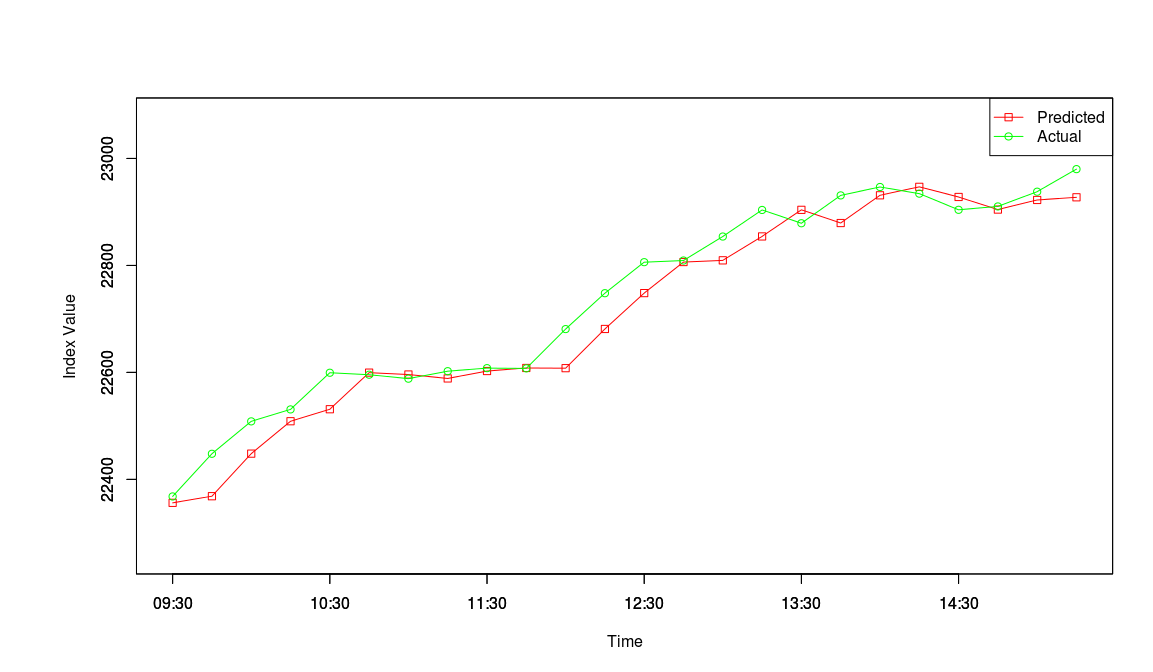
\includegraphics[scale = 0.3]{pictures/predictionResult.png}
\label{fig:error_plot}
\end{figure*}


In order to determine the prediction accuracy of our model we use 2 metrics. 

\begin{enumerate}
\item \textbf{Normalized Mean Square Error (NMSE)}

The Normalized Mean Square Error is used to predict the accuracy of our index prediction. It is calculated as - 
\begin{equation}
NMSE = \frac{\sum_{t=1}^{N} (O_t - P_t)^2}{\sum_{t=1}^N (O_t - \bar{O_t})^2}
\end{equation}

where, $t$=[1,N] are the time series points on which values are predicted. $O_t$ and $P_t$ are the Original Value and the Predicted Value at time $t$ respectively. $\bar{O_t}$ is the mean of the original values. This gives us the difference between our prediction results.

\item \textbf{Sign Correctness Percentage (SCP)}

This is used to evaluate the performance of the directional prediction. The number of times the model can predict the direction in which the market is about to turn. It is calculated as -
\begin{equation}
SCP = \frac{\{ Sign(P_t) = Sign(O_t) | t = 1,2,...,N\}}{N} \times 100
\end{equation}
\end{enumerate}

The table-\ref{tab:performance} gives the result obtained by running our method on the 35 day stock data collected by us spread over a 10 week span. We give the average NMSE and SCP values of each week trading. 



\subsection{Trading Engine}
A trading engine is used to simulate trading in stock market according to our predictions and the return value for trade in the stock market is found out. 

In a highly liquidated market, the 2 main trading strategies used for stocks are - 
\begin{enumerate}
\item Buying of rising stocks, where the stocks are bought at the current value and later sold at a higher value for a profit value.
\item Short selling of Stocks, stocks which are not currently owned by a trader and will be bought later from the open market at a lower price than current price, thus resulting a profit.
\end{enumerate}

We follow the popular Lavrenko's trading strategy as introduced in \cite{lavrenko2000language}. According to the trading strategy, whenever we see a \textit{positive} trend in the market Rs. 10,000 worth of stocks is bought. The trader holds the stocks for 1 hour and then sells it. If during the 1 hour a profit of 1\% can be done then the stocks are sold immediately. If the trend is \textit{negative} Rs. 10,000 worth of stocks is short-selled. Again after 1 hour time or if 1\% lower price is conceived then the stocks are bought back. At the end of 1 hour the stocks are traded even if loss has to be faced by the trader. Assumptions taken are that the stock transaction costs are zero. 


We do trading on the stocks of \textit{Tata Steel} traded in BSE as \textbf{BOM:500470} in the steel sector. We compare our trading return with those of \cite{Hagenau:2013} in table-\ref{tab:return} and show the comparison of  trade return with similar trading parameters in figure-\ref{fig:trade} . 

\begin{figure*}[htbp]
\centering
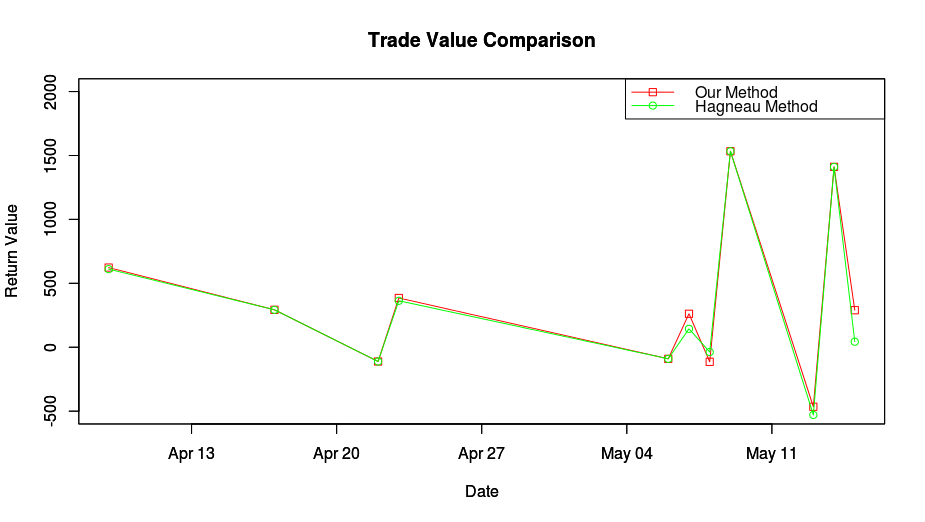
\includegraphics[scale = 0.4]{pictures/tradeReturn.png}
\caption{Stock Simulated Trade Return}
\label{fig:trade}
\end{figure*}

\begin{table}[htbp]
\centering
\caption{Trade Percentage Return}
\label{tab:return}
\vspace{15pt}
\begin{tabular}{|c|c|}
\hline
Our Method                   & Hagneau et al. \cite{Hagenau:2013}              \\ \hline
\multicolumn{1}{|r|}{3.65\%} & \multicolumn{1}{r|}{3.3\%} \\ \hline
\end{tabular}
\end{table}

Our method shows better almost similar and in some cases better trading returns for simulated trading as in figure-\ref{fig:trade} rather than the one used in \cite{Hagenau:2013}. This shows how our model is more useful for stock trading and gives better trade return. 


\section{Conclusion}
\label{sec:conclusion}\textbf{}

Our research shows that due to the changing nature of nature a static feature space is not a good choice, and dynamic feature spaces give better results. We have designed a prediction model for the forecasting of the trading index, and we develop a trading system according to the index prediction. 

A dynamic lossless homogeneous feature space change conversion method is designed. This changes the feature space of the clustering model every time. Features are extracted according to the importance of the word in the current news items. 

The forecasting system uses projected clustering in order to overcome the \textit{Curse of Dimensionality}. The Projected clustering is used for classification of the news documents, which will help predict the trend of the stock market in the next time frame. The projected clustering uses fading cluster structures which help define the way importance of old news gets reduced over time.

Finally with the use of an Artificial Neural Network we predict the BSE S\&P 500 Sensex index value is predicted. The change in the Index value is used to predict the trend in the market and stocks are traded according to these trends. We compare our method with the existing research in \cite{Hagenau:2013}. Our simulated trading system shows better percentage return results than the existing method. Thus our model gives a better trading result.

The method designed in this work can be further investigated in the following ways- 
\begin{enumerate}
\item To capture the concept drift, we have used projected clustering with dynamic feature space. Ensemble Classifiers is also a promising way to capture concept drifts in data streams. Our method can be used with this to see the nature of the change.

\item Our method uses all kinds of news to predict trends. However when we are predicting a particular stock, a model to track the individual sector trends can also be used alongside for better predicting trends relevant to a particular stock.
\end{enumerate}
\section*{References}
\bibliographystyle{elsarticle-harv}
\bibliography{references}
\end{document}